% !Mode:: "TeX:UTF-8"

\chapter{基于关系挖掘和预测的代码变更影响分析}

%%%%%%%%%%%%%%%%%%%%%%%%%%%%%%%%%%%%%%%%%%%%%%%%%%%%%%%%%%%%%%%%%%%%%%%%%%%%%%%
\section{引言}

软件变更是软件维护的核心环节。对软件系统的修改可能引发系统其他部分的不良副作用或连锁反应。而变更影响分析的目标在于识别变更的涟漪效应,帮助开发者安全地进行变更。方法之间的变更影响可以分为以下两种类型:

(1)依赖型变更影响关系:依赖型指的是能直接体现在代码静态结构中的变更影响关系,如将项目代码组织为抽象语法树、系统依赖图或影响图,通过图结构的可达性分析等方法,得到的静态依赖关系。方法间的依赖型变更影响关系表现为方法间的调用或间接调用关系。

(2)逻辑型变更影响关系:在这种类型的变更影响关系中,方法之间不存在静态结构之间的关联关系,但它们的实现逻辑或所操作的数据之间存在某种隐含的关联。具体来说,这种关系可能源于它们共同维护某个数据的一致性、共享某些资源,或其功能逻辑有某种预期联系。因此,当某个方法发生变化时,可能会间接影响到其他方法的行为或结果。

依赖型影响关系可在代码的静态结构中直接显现,通过基于依赖关系的传统影响分析方法甚至开发工具即可捕捉,而逻辑型影响关系通常只能通过开发者通过阅读代码进行人工分析,不仅分析难度大,还往往难以被开发者察觉,是导致维护时出现功能性问题的主要原因之一。正是由于逻辑型影响的存在,开发者在维护软件代码时面临着诸多困扰,会出现难以理解软件架构、难以安全进行代码变更等问题。


为了解决上述问题,本文以C/C++项目为研究对象,针对不同的应用场景,实现了基于依赖闭包、基于克隆检测以及基于共现关系挖掘的的变更影响分析方法,在研究这三种方法各自的优点和局限性的基础上,提出了基于代码预训练模型的变更影响预测方法,并通过实验验证了基于代码预训练模型的方法的有效性。


\section{代码预处理和中间表示生成}

为了便于后续分析,需要对项目源代码进行预处理,将其转换为适合后续方法处理的中间表示。本文首先将项目源代码解析为抽象语法树(Abstract Syntax Tree, AST),并在此基础上进一步提取方法调用链以及全局变量的定义-使用链,为后续的变更影响分析奠定基础。

\subsection{基于clang的抽象语法树生成}
抽象语法树把代码的语法结构以树形的方式进行了抽象化描述。在这个树形结构中,每一个节点都对应着代码中的某个元素,比如变量声明、语句或者是表达式等。从抽象语法树的根节点出发,代码逐步被拆解成更小的部分,直到最终到达叶节点,这些叶节点代表了代码中最基本的元素,如操作符或变量等。AST 能够清晰地展示出代码的层次和结构,为编译器或其他工具分析和处理代码提供便利。


Clang 是由苹果公司发起的支持 C、C++、Objective-C 和 Objective-C++语言的编译器前端,负责对代码进行词法分析、语法分析和语义分析,对程序代码的分析和理解至关重要\cite{clang}。而libclang 是 Clang 编译器的一个重要组成部分,它提供了一套用于解析源代码的程序接口。这些程序接口允许开发者在项目中使用 Clang 的强大语言解析和代码分析功能\cite{libclang}。本文使用libclang 生成AST ,提取代码中的调用和依赖关系,为后续进一步分析提供基础。

在 libclang 解析得到的抽象语法树中,游标(cursor)是一个核心概念,它作为一个指针或引用存在,每个 cursor 都与 AST 中的一个特定节点相对应,表示了源代码中的一个结构元素。通过操作 cursor,可以遍历整个 AST,访问和分析代码中的各种元素,如获取变量的类型、方法的参数列表、类的成员等。libclang 提供了一系列 API 函数来操作 cursor,例如:遍历 AST 中的 cursor、获取 cursor 的类型(如是否为方法定义、变量定义、变量引用等)、获取 cursor 所代表的源代码元素的名称、类型、位置等信息、获取 cursor 的父节点或子节点等。

\begin{table}[htbp]
\caption{重要AST节点类型标识}
\label{1_重要AST节点类型标识}
\vspace{0.5em}\centering\wuhao
\begin{tabular}{cc}
\toprule
节点标识 & 含义  \\
\midrule
Translation\_Unit & 一个翻译单元 \\
Function\_Decl  & 方法定义 \\
Parm\_Decl & 方法的参数定义 \\
Var\_Decl & 变量定义 \\ 
Devl\_Ref\_Expr  & 变量引用  \\
Call\_Expr  & 方法调用  \\
\bottomrule
\end{tabular}
\end{table}   

本文通过操作游标,遍历 AST,获取整个 AST的结构以及重要节点的详细信息,在此之上进一步提取代码元素之间的关系。clang定义的部分重要节点类型如表\ref{1_重要AST节点类型标识}中所示。值得注意的是,在 clang 中是不区分方法声明和方法定义的,统一用 Function\_Decl来标识,区分二者主要看是否有方法体,在 libclang 中提供了程序接口供开发者调用以进行区分。

\subsection{方法调用链提取与分析}
为了进行方法调用链提取与分析,在使用 libclang 提取代码的抽象语法树后,遍历整棵树来提取方法之间的调用关系。本方法重点关注抽象语法树上的方法节点,以及方法节点内部的调用节点,分别对应着代码中方法的定义和方法内部对其他方法的调用。

\begin{algorithm}[htbp]
    \caption{方法调用链提取}
    \label{1_方法调用链提取}
    \KwIn{项目中的所有代码文件: $files$}
    \KwOut{方法摘要表: $functions$}
    \SetKwFunction{scanAndAnalyze}{scanAndAnalyze}
    \SetKwFunction{traverse}{traverse}
    \SetKwProg{Fn}{Function}{:}{}
    
    \Fn{\scanAndAnalyze{$files$}}{
        $functions \gets \{\}$ \tcp*[h]{初始化方法摘要} \;
        \ForEach{$file \in files$}{ \tcp*[h]{第一次遍历:收集方法的定义} \;
            $cursor \gets \text{libclang.parse}(file).cursor$ \tcp*[h]{获取AST的根游标} \;
            traverse($cursor$, 0, $functions$, $file$, True) \tcp*[h]{遍历AST,收集方法定义} \;
        }
        \ForEach{$file \in files$}{ \tcp*[h]{第二次遍历:分析方法调用情况} \;
            $cursor \gets \text{libclang.parse}(file).cursor$ \tcp*[h]{获取AST的根游标} \;
            traverse($cursor$, 0, $functions$, $file$, False) \tcp*[h]{分析方法调用} \;
        }
        \textbf{return} $functions$ \;
    }
    
    \Fn{\traverse{$node, depth, functions, filePath, isFirstScan$}}{
        \If{$isFirstScan$}{
            \If{$node.kind == \text{CursorKind.FUNCTION\_DECL}$}{
                $function \gets \text{collectionInfo}(node)$ \tcp*[h]{收集方法信息} \;
                $functions.\text{add}(function)$ \tcp*[h]{将方法添加到方法摘要} \;
            }
        }
        \ElseIf{$node.kind == \text{CursorKind.CALL\_EXPR}$}{
            parse($node$) \tcp*[h]{分析被调用的方法} \;
        }
        \ForEach{$n \in node.get\_children()$}{
            traverse($n$, $depth + 1$, $functions$, $filePath$, $isFirstScan$) \tcp*[h]{递归遍历子节点} \;
        }
    }
\end{algorithm}



方法调用链提取流程如算法\ref{1_方法调用链提取}所示。对抽象语法树的遍历主要分为两次,第一次遍历的目的是获取所有的方法定义。首先提取所有的Function\_Decl 节点,它表示方法的定义,在该节点中可提取方法签名。在Function\_Decl 节点下,提取子节点 Parm\_Decl,该节点表示方法的参数列表,在该节点中可提取参数名称和参数类型等参数相关信息。然后提取Function\_Decl节点的子节点 VarDecl,该节点表示在该方法内定义的局部变量。在对方法进行分析时,我们本身不关心方法的内部实现,但是由于在 C/C++语言中,存在局部变量可以和全局变量重名的情况,在这里提取方法内定义的局部变量,方便后续在提取全局变量的使用时,排除同名局部变量的影响。除此之外,还需提取整个方法的 token 序列,所在文件以及作用域。


第二次遍历的目的是提取方法之间的调用关系。提取 Function\_Decl 节点
的子节点 Call\_Expr,该节点标签表示的是调用语句,可提取调用的方法名。注意,由于主要分析该项目中由开发者定义的方法之间的依赖关系,所以对于一些标准库方法的调用选择忽略,不进行提取。

分析结束后,将会获得每个方法的方法调用关系和详细信息,将提取到的信息组织为一个方法摘要表,表的每一项表示一个方法的摘要,每个摘要由\textless \textit{funcID}, \textit{token}, \textit{params}, \textit{call}, \textit{scope}, \textit{file}, \textit{localvar} \textgreater 共7部分组成,分别表示方法的唯一ID标识,方法体,方法参数列表。方法内调用的其他方法,方法的作用域,方法所在模块和方法定义的局部变量。


\subsection{全局变量定义-使用链提取与分析}
在C/C++代码中,相同描述符修饰下的全局变量的定义、作用域、生命周期和方法是同级别的,所以在本文中,将全局变量也作为独立的代码单元进行分析。
全局变量定义-引用链的提取和方法的定义和调用提取类似,对 AST 的遍历主
要也分为两次。
% 具体流程如图\ref{1_全局变量提取流程图}。

% \begin{figure}[h]
% \centering
% 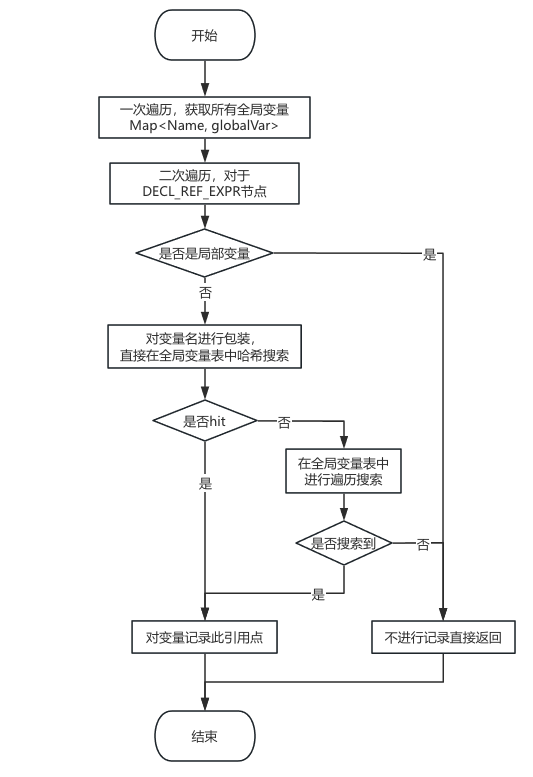
\includegraphics[width = 0.7\textwidth]{全局变量提取流程图.jpg}
% \caption{全局变量提取流程图}
% \label{1_全局变量提取流程图}
% \end{figure}

第一次遍历获取所有的全局定义。首先提取所有的
Var\_Decl 节点,它表示变量定义,然后提取节点中的变量名和变量类型。注
意,由于在 AST 中的节点标签中无法区分变量是否是全局的,所以这里根据节点在 AST
中的深度来判断是否是全局变量,并且在变量名前加上针对该项目文件的绝对路径,来
保证变量名的唯一性。在确定其为全局变量后,还需进一步提取该变量的作用域。在
C/C++语言中,static关键字可用于修饰变量和方法,意味着该变量或该方法只能在其所在文
件内使用,而不是全局可用,因此需要对其作用域进行判断。一次遍历提取到的结果是
一个全局变量表,这里使用哈希表 Map<Name, globalVar>的数据结构进行存储,方便对
全局变量进行查找。

第二次遍历的主要目的是提取全局变量的引用点。在方法节点子树中搜索
Devl\_Ref\_Expr 节点,该类型节点表示对变量的引用,这里首先判断被引用的变量是否是局部
变量,根据方法摘要表中该方法的相关信息可以判断,如果是则直接返回,因为我们不关心方法内的局部变量引用。如果不是,则证
明使用的是全局变量,首先在哈希表中进行查找该变量名,以节省检索时长,如果查找到了,说明
是在该文件中定义的全局变量,同时能够保证被 static 修饰的全局变
量的判断的准确性。如果没有查找到,则说明引用了别的文件中定义的全局方法,则在哈希
表中进行遍历查找,记录该全局变量被引用的方法。

分析结束后,将全局变量的信息组织为全局变量信息表,表的每一项表示一个全局变量的信息,每条信息由\textless \textit{globalVarID}, \textit{type}, \textit{use}, \textit{scope}, \textit{file}  \textgreater 共5部分组成,分别表示全局变量的唯一ID标识,变量类型,变量的引用点所在的方法,变量的作用域以及变量所在模块。



\section{基于依赖闭包的变更影响分析}

依赖关系传递闭包方法是一种基于静态依赖关系的技术手段,通过识别代码模块间的关联性划定受变更影响的范围\cite{2022An}。其核心思想是利用依赖关系的传递性,通过构建和分析依赖图,揭示所有可能受到影响的代码模块或单元\cite{2021Improving}。该方法主要分为以下两步。

\noindent \textbf{1. 构建依赖关系图}
\label{1_代码依赖图}



以抽象语法树、全局变量信息表和方法摘要表为基础,构建程序的依赖关系图。本文的依赖关系图是对简单调用图的扩展,增加了方法和全局变量之间的引用关系,方便后续的分析。图节点代表代码中的基本元素,本文中是方法和全局变量,而边则表示这些元素之间的依赖关系。依赖关系包括方法调用和全局变量变量引用,在全局变量信息表和方法摘要表中可直接提取依赖关系。生成边的原则如下:
\begin{itemize}
    \item 调用边(call):方法间的调用关系。如果方法A调用了方法B,在图中增加一条从节点A指向节点B的有向边。
    
    \item 引用边(use):方法和全局变量的引用关系。如果方法A引用的全局变量C,在图中增加一条从节点A指向节点C的有向边。
\end{itemize}


\begin{figure}[htbp]
    \centering
    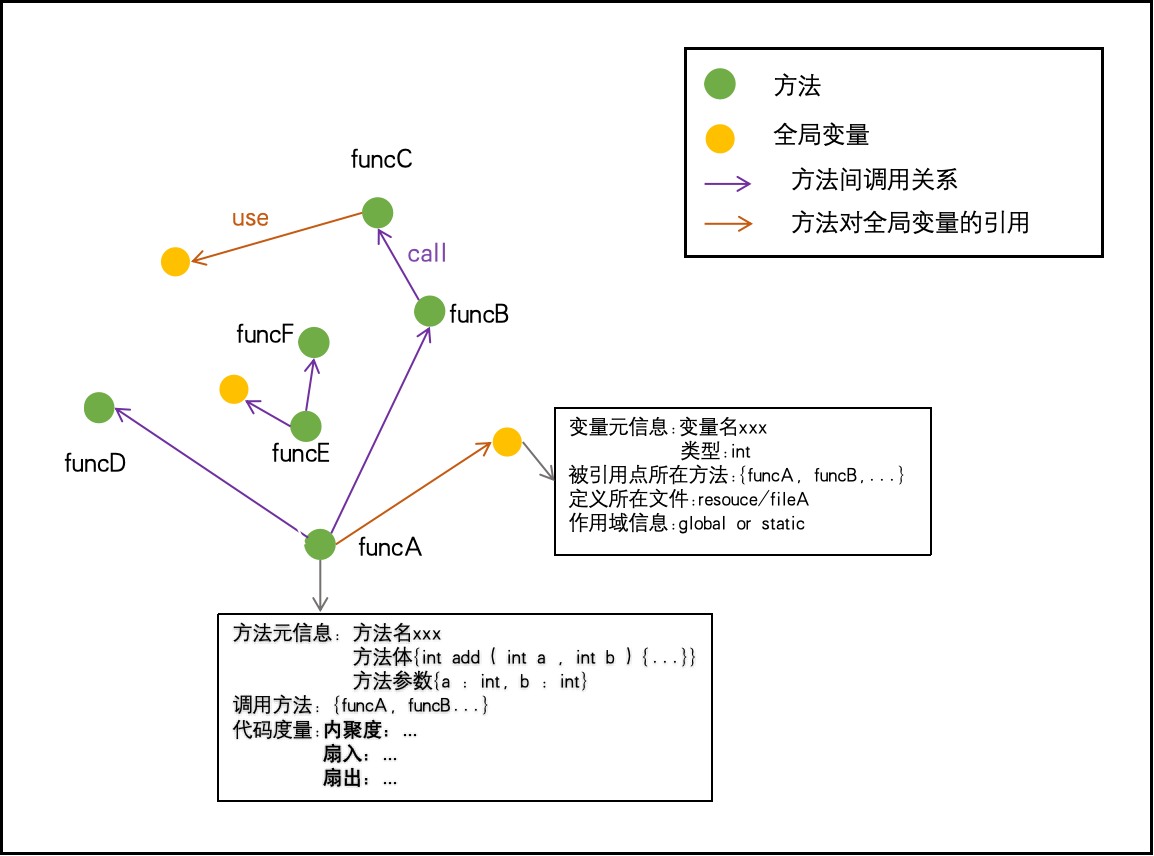
\includegraphics[width = 0.7\textwidth]{figures/依赖关系图.png}
    \caption{依赖关系图示例}
    \label{1_依赖图示例}
    \end{figure}


通过这种方式,依赖关系图不仅能够系统地表示代码中各个元素之间的直接依赖关系,还能为后续的变更影响分析提供结构化的图形模型。如图\ref{1_依赖图示例}为依赖关系图示例,该图中共有6个方法和3个全局变量,其静态依赖关系如图中的边所示。


\noindent \textbf{2. 执行变更影响分析}

这一过程旨在确定哪些方法在代码变更时可能受到影响,以及这些影响的传播路径。本文以方法为研究对象,以变更类型为方法变更\cite{DZBZ202104016},基于方法和方法之间的以下两种关系RBM(relationships between methods)对每一个方法识别当其变更时受影响的方法集IMS(impacted method set),定义如式\ref{1_RBM}所示,以方法f和方法g的关系为例,CALL方法和RETURN分别代表f和g的调用和被调用关系。
\begin{equation}
\begin{array}{l}
\label{1_RBM}
R B M=C A L L \cup R E T U R N \text { where } \\
(f, g) \in C A L L \Longleftrightarrow f(\text { transitively)calls } g, \\
(f, g) \in R E T U R N \Longleftrightarrow f(\text { transitively)returns into } g
\end{array}
\end{equation}

对于依赖关系图中的每个节点,计算该节点的传递闭包。传递闭包是指从某个特定节点出发,根据上文定义的依赖关系和图的可达性,可以直接或间接到达的所有节点的集合,反映了节点之间的依赖链以及影响传播的范围。传递闭包的具体迭代模型如下:
% \begin{equation}
% \begin{array}{l}
% \label{1_IMS}
% I M S^{(N)}=I M S_{C A L L}^{(N)} \cup I M S_{R E T U R N}^{(N)} \\
% I M S_{ {RETURN }}^{(N+1)}=\bigcup_{define \in (I M S_{R E T U R N}^{(N)}-I M S_{R E T U R N}^{(N-1)} ) } I M S({ define }) \\
% I M S_{C A L L}^{(N+1)}=\bigcup_{ {define } \in (I M S_{C A L L}^{(N)})} I M S( { define }){, define } \in \\
% \left(I M S_{C A L L}^{(N)}-I M S_{C A L L}^{(N-1)}\right) 
% \end{array}
% \end{equation}
\begin{equation}
\begin{array}{l}
\label{1_IMS}
I M S^{(N)}=I M S_{C A L L}^{(N)} \cup I M S_{R E T U R N}^{(N)} \\
I M S_{ RETURN }^{(N+1)}=\bigcup_{define \in (I M S_{R E T U R N}^{(N)}-I M S_{R E T U R N}^{(N-1)} ) } I M S_{RETURN}({ define }) \\
I M S_{C A L L}^{(N+1)}=\bigcup_{ define  \in (I M S_{C A L L}^{(N)}-I M S_{C A L L}^{(N-1)})} I M S_{CALL}( { define })
\end{array}
\end{equation}


其中N表示第N轮迭代,第N+1轮的迭代受N和N-1轮的影响,反映出软件系统中的变更的涟漪效应。为了高效地计算传递闭包,使用广度优先搜索遍历图中的各个节点及其依赖边,进而识别出所有直接或间接依赖于某个节点的其他节点。每次从某个节点出发时,都会跟踪并记录通过依赖关系可到达的所有节点,,最终得到的节点集合中,所有的节点都与初始变更的节点存在某种直接或间接的依赖关系。这些方法可以视为受变更影响的范围,意味着它们在该方法变更后,可能会因为依赖关系的传递而受到影响。通过这一分析,我们不仅可以识别出受影响的直接方法,还能揭示出那些通过多次间接依赖而受到影响的方法,帮助开发者全面了解变更的潜在影响范围。


在图\ref{1_依赖图示例}的例子中,方法 funcA 调用了 funcB 和funcD,funcB 调用了 funcC。在对 funcB 进行变更影响分析时,会直接影响到 funcA和funcC,根据依赖关系闭包,会间接影响到funcD。所以与 funcB 有变更影响关系的方法集合为\{funcA, funcC, funcD\} 。


\section{基于克隆检测的变更影响分析}
代码克隆(Code Clone)是指在代码中存在两段或多段内容相似或完全相同的代码片段。因此它们在逻辑上往往具有相同的功能或行为。如果对其中一个克隆片段进行了变更(例如修复了一个 bug、添加功能或进行优化),那么在其他地方相同或相似的代码也可能需要同步修改,否则可能会导致系统的不一致性或错误,这是典型的逻辑型变更影响。

\begin{figure}[htbp]
\centering
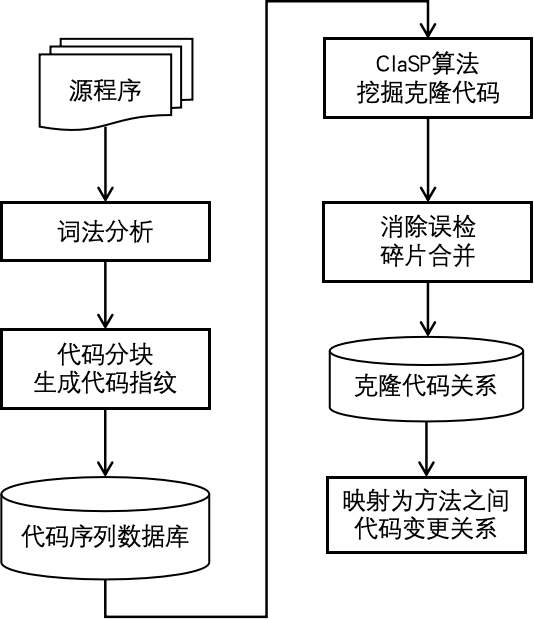
\includegraphics[width = 0.4\textwidth]{代码克隆流程}
\caption{基于克隆检测的变更影响分析方法流程}
\label{1_基于代码克隆的变更影响分析方法流程}
\end{figure}

基于克隆检测识别变更影响的方法在文献\cite{daipeng2024software}中首次被提出。本文不同于该方法使用机器学习方法进行克隆检测,而是以方法为研究对象,使用频繁模式挖掘技术,以求对克隆代码得到更精准的检测。该方法主要分为两步,首先对源程序进行预处理,通过代码分段及代码指纹提取的方式对源程序进行编码,生成代码序列数据库。随后利用频繁模式挖掘算法ClaSP得到克隆代码列表,具体的处理流程如图\ref{1_基于代码克隆的变更影响分析方法流程}所示。


\noindent \textbf{1.代码预处理}

(1)词法分析。词法分析的主要步骤分为以下几步:

\begin{itemize}
    \item 去除注释:注释通常用于解释代码的意图,并不直接影响程序的执行,但不同的代码实现中注释内容可能存在差异,这会导致本质相同的代码片段由于注释的不同而被误判为非克隆。
    
    \item 去除头文件引用语句:源代码文件往往包含多个头文件,而不同的源文件可能引用相同的头文件。如果不对头文件进行统一的处理,算法可能在不同的源文件中检测头文件引用的代码克隆情况,影响克隆检测的效率和准确性。
    
    \item 程序标准化:为了避免因变量名的变化导致漏检,在方法内部对变量名进行统一标准化处理。

\end{itemize}

(2)代码分块。这一步将代码拆解成更小、更易于对比的单元,从而提高克隆检测的准确性。本文的代码分块策略按代码结构的不同分为几类:

\begin{itemize}
    \item 顺序结构:按固定行数分块,行数可由用户定义,默认为6行一块。行数越小则识别结果越精准,越能识别更细小的代码克隆情况。
    
    \item 控制结构:将选择结构(if、then、else、endif、switch)、循环结构(while、for)、和域结构(\{、\})共同描述为控制结构,识别并根据对应的关键分块词进行分块。这是由于控制语句是代码逻辑的重要分界点,将它们作为分块的标准可以确保检测系统能聚焦于实际功能的逻辑边界。
\end{itemize}

值得注意的是,分块时大括号不被视为代码块的一部分。不同的开发者在代码排版上可能存在差异,例如有的开发者将大括号置于同行,而另一些则习惯将大括号另起一行。为了避免这种格式差异对克隆检测结果产生干扰,大括号被排除在代码块之外。

(3)代码指纹提取。遍历代码块的每一行语句,将每行语句转化为数字序列,再将所有数字序列合并,转化为代码块的“指纹”。该指纹将代表代码片段,用于识别代码片段之间的相似性或重复性。鉴于哈希算法在计算上的高效性与实现的简便性,它在生成代码指纹方面具有显著的优势。因此,本文选择采用冲突率较低的hashpjw算法提取代码指纹。

\noindent \textbf{2.基于克隆检测的变更影响关系提取}

序列数据挖掘(Sequence Data Mining,SDM)是时序数据挖掘领域的一个重要研究方向,旨在从给定的输入数据库中,探索在大量对象之间随顺序频繁出现的模式。判断一个模式是否具有意义的阈值被称为最小支持度。本文中,将代码指纹片段作为序列,合并起来为序列数据库,利用序列数据挖掘算法,检测频繁出现的模式,从而将问题转化为闭合序列挖掘问题。这里对于数据挖掘的一些基本概念不再赘述,具体可参考文献\cite{2013ClaSP}。具体的流程分为以下两步:

(1)基于闭合频繁子序列挖掘算法的代码克隆检测。首先生成频繁序列,作为频繁闭合序列的候选FCC(Frequent Closed Candidates)。第二步执行剪枝,从候选中剔除所有非闭合的序列,最终得到精确的FCS(Frequent Closed Set)。主要的流程如算法\ref{1_ClaSP算法}所示,接下来是对该算法的详细解释。

\begin{algorithm}
\caption{ClaSP算法}
\label{1_ClaSP算法}
\KwIn{序列数据库}
\KwOut{频繁闭合序列集 $FCS$}
 $F_1 \gets \{\text{频繁 1-序列}\}$ \\
 $FCC \gets \emptyset$, $FCS \gets \emptyset$  \\
\For{\textnormal{all} $i \in F_1$}
{
    $F_{ie} \gets \{\text{频繁 1-序列的长大于i的扩展序列 } \}$ \\
    $FCC_i \gets \text{DFS-Pruning}(i, F_1, F_{ie})$ \\
    $FCC \gets FCC \cup FCC_i$
}

 $FCS \gets \text{N-ClosedStep}(FCC)$
\end{algorithm}

ClaSP(Closed Sequential Patterns algorithm)算法由Gomariz等人\cite{2013ClaSP}提出,兼具高效性和准确性的优点。在该算法中,首先找到所有的频繁的1-序列(即长度为1的序列),然后,对于所有频繁的1序列,通过DFS-Pruning 算法递归地探索相应的子树。DFS-Pruning 算法通过递归生成候选模式(包括 s-扩展和 i-扩展,分别在模式末尾和任意位置添加新元素)并检查其支持度,返回以当前模式 $p$ 为前缀的所有频繁模式集。对所有频率为1的序列进行此处理,得到FCC。

最后去除FCC中出现的非闭合序列。通过检查对应模式的子序列和超序列的支持度,将序列的节点进行合并,防止继续遍历冗余节点。最终得到的FCS即为所有克隆代码集。

(2)基于克隆代码碎片合并提取方法间的变更影响关系。由于先前的代码分段处理导致克隆代码呈现为片段间的克隆关系,为了恢复代码的完整性,进一步对这些碎片进行合并。基于每段代码的位置信息,将属于同一方法的碎片进行整合,重建为方法间的克隆关系。通过这种方式,最终得到的是方法与方法之间的克隆关系,反映了不同方法之间在代码修改过程中的潜在影响,即方法间的变更影响关系。

\section{基于共现关系挖掘的变更影响分析}

在软件工程中,分析代码变更历史是理解软件演化重要手段之一。在开发者对项目进行维护的过程中,通常是以一个提交(commit)为单位进行功能上的变更。当进入新的维护工作时,如对同一功能进行升级等,通常的做法是参考前人的开发历史,对当前开发工作做指导,以防止变更的不完全。基于这一特点,本文实现了基于变更历史和共现关联关系的变更影响分析方法,分析对象是软件项目的变更历史。该方法能够提取蕴含在代码变更历史中的变更影响关系,尤其适用于具有丰富变更记录的软件项目。

该方法的核心原理是在代码变更历史中,频繁同时更改的代码片段,通常存在着某种潜在的变更影响关系。这种变更影响关系不仅仅局限于静态结构上的依赖,还包括功能上的耦合和实现上的相互作用。因此,通过对这些历史变更数据的深入挖掘和分析,我们可以揭示出更丰富的逻辑型变更关系。

\noindent \textbf{1.基于代码变更历史提取的序列数据库构建}

由于 Git 是现代软件开发中最广泛使用的版本控制工具,因此,本文的分析主要基于由 Git 进行版本管理的项目。具体步骤如下:

\begin{itemize}
    \item 收集项目代码库及变更历史记录。克隆项目的代码库到本地,通过git log命令获取所有的commit,包括每个提交的哈希值commitHash等信息。
    \item 提取每个提交的变更信息。对每个提交运行git show <commitHash>命令,查看该提交引入的代码变更(即“diff”或差异),这会显示哪些文件被修改、添加或删除,本文主要关注标记为“修改”的文件,这些修改的文件中包含了具体的代码变化,即代码行的增、删、改操作,记录该commit引起的所有发生变更的代码行。
    \item 定位变更代码行所属的方法。通过libclang分析变化前文件得到的抽象语法树可获取每个方法对应的代码行,与变更的代码行位置进行匹配,得到变更的代码行所在的方法。
    \item 提取变更方法与提交的关系。对于每个提交,提取出所有受影响的方法(即发生变化的方法),并将这些方法构成一个变更方法列表,用Map<commitID, List<Methods>>的结构存储每个commit变更的方法,作为序列数据库,便于后续分析与处理。
    
\end{itemize}

\noindent \textbf{2.基于共现关系挖掘的变更影响关系提取}

基于关联规则(Association Rules)的共现关系挖掘方法是反映事物之间相互依存性和关联性的一个重要数据挖掘技术,旨在从大量数据中挖掘出有价值的项之间的相关关系。共现关系可以视为关联规则的一种表现形式,它描述了在给定集合中,某一组项(或特征)经常出现在同一事务中。例如,在零售分析中,常见的共现关系是“购买了面包的顾客通常也会购买牛奶”。在这种情况下,“面包”和“牛奶”是一对共现项。在本文的代码变更影响分析中,共现关系描述的是在一次提交中,哪些方法经常同时发生变更。如果两个方法在多个提交中频繁一起变动,则它们之间可能存在某种依赖关系或变更影响关系。

\begin{algorithm}[h]
    \caption{频繁共现变更方法对挖掘算法}
    \label{同时变更方法对挖掘算法}
    \KwIn{序列数据库 $D$, 支持度阈值 $min\_sup$, 置信度阈值 $min\_conf$}
    \KwOut{变更影响方法对 $change\_impact\_pairs$}
     $F_1 \gets \emptyset$  \# 频繁1项集\\  
    \For{all $f \in D$} {
        \If{support$(f) \geq min\_sup$} {
            $F_1 \gets F_1 \cup f$
        }
    } 
    $F_2 \gets \emptyset$  \# 频繁2项集\\ 
    \For{all $(f_1, f_2) \in P = \{ (f_i, f_j) \mid f_i, f_j \in F_1, i \neq j \}$} {
        \If{$\text{Support}(f_1, f_2) \geq min\_sup$} {
            $F_2 \gets F_2 \cup (f_1, f_2)$
        }
    }
    
    $change\_impact\_pairs \gets \emptyset$ \\ 
    \For{all  $(f_1, f_2) \in F_2$} {
        \If{confidence$(f_1, f_2) \geq min\_conf$} {
            $change\_impact\_pairs \gets change\_impact\_pairs \cup (f_1, f_2)$
        }
    }
    \Return{$change\_impact\_pairs$}
    \end{algorithm}


常用的频繁项集的评估标准有支持度和置信度。支持度表示共现项在数据集中出现的次数占总数据集的比重,用于衡量一组项在数据集中的普遍程度。在代码变更分析中,支持度表示某一方法对在多个提交中同时出现的频率,计算公式如下:

\begin{equation}
\label{1_Support}
Support(funcA,funcB)=\frac{num(AB\text{共现})}{num(AllCommits)}
\end{equation}

置信度表示共现项中一个出现后,另一个项出现的概率。变更分析中,置信度度量表示当方法A被修改时,方法B被修改的概率,计算公式如下:

\begin{equation}
\label{1_Confidence}
Confidence(funcA\Leftarrow funcB)=\frac{P(AB\text{共现})}{P(B\text{出现})}
\end{equation}

在前文所述的基础上,本文设计了如算法\ref{同时变更方法对挖掘算法}所示的频繁共现变更方法对挖掘算法,算法的基本思想是通过挖掘在序列数据库中(即代码提交历史中)中的共现关系,计算得到频繁同时变更的方法对,这样的关系表明它们在变更过程中有着较为显著的相互依赖关系,反映了方法间的变更影响关系。

\section{基于代码预训练模型的变更影响预测}
\subsection{研究动机}

尽管前文所述的方法在一定程度上能够进行变更影响分析,但它们仍然存在一些局限性,主要表现在以下几个方面:

\begin{itemize}

    \item 冷启动问题:当项目代码拥有丰富的变更历史时,可以通过共现关系挖掘方法提取具有变更影响关系的方法,然而,并非所有软件项目都具备足够的变更历史支持。例如,新项目或缺乏完善版本管理的项目中,历史变更数据的匮乏使得该方法难以发挥作用。

    \item 影响类型覆盖不全:在仅有项目源代码的情况下,共现关系挖掘方法无法直接应用,而仅依赖基于依赖闭包和基于克隆检测的方法,虽然能够识别部分影响关系,但对逻辑型变更影响的挖掘仍显不足。逻辑型影响关系往往是系统中隐蔽性最强,同时对功能正确性威胁最大的部分,其难以被捕获的特性极大限制了现有方法的适用性。
    
    \item 影响模式难以迁移:共现关系挖掘方法只能从历史变更中学习已经出现的影响关系,而对于未发生变更的方法,无法有效将已知的影响模式迁移到新的场景中。这种局限性导致模型的通用性和适应性不足,尤其在开发者希望预判未来变更影响时,难以提供可靠的支持。
    
\end{itemize}


针对上述问题,本文提出一种基于代码预训练模型的变更影响预测方法。该方法通过整合前述的依赖闭包、克隆检测和共现关系挖掘方法,构建具有代表性的数据集,并对数据进行清洗和增强,通过微调代码预训练模型用于变更影响关系的预测。这种方法不仅能够弥补历史数据不足的问题,还能通过模型的语义理解能力覆盖更广泛的影响类型。通过这一方法,本文旨在提高变更影响分析的全面性和准确性,为复杂软件系统的维护提供更有力的支持。


\subsection{整体流程设计}

针对上述问题,本文提出一种基于代码预训练模型的变更影响预测方法,整体流程设计如图\ref{2_基于代码预训练模型的变更影响预测方法框架}所示。

\begin{figure}[htbp]
\centering
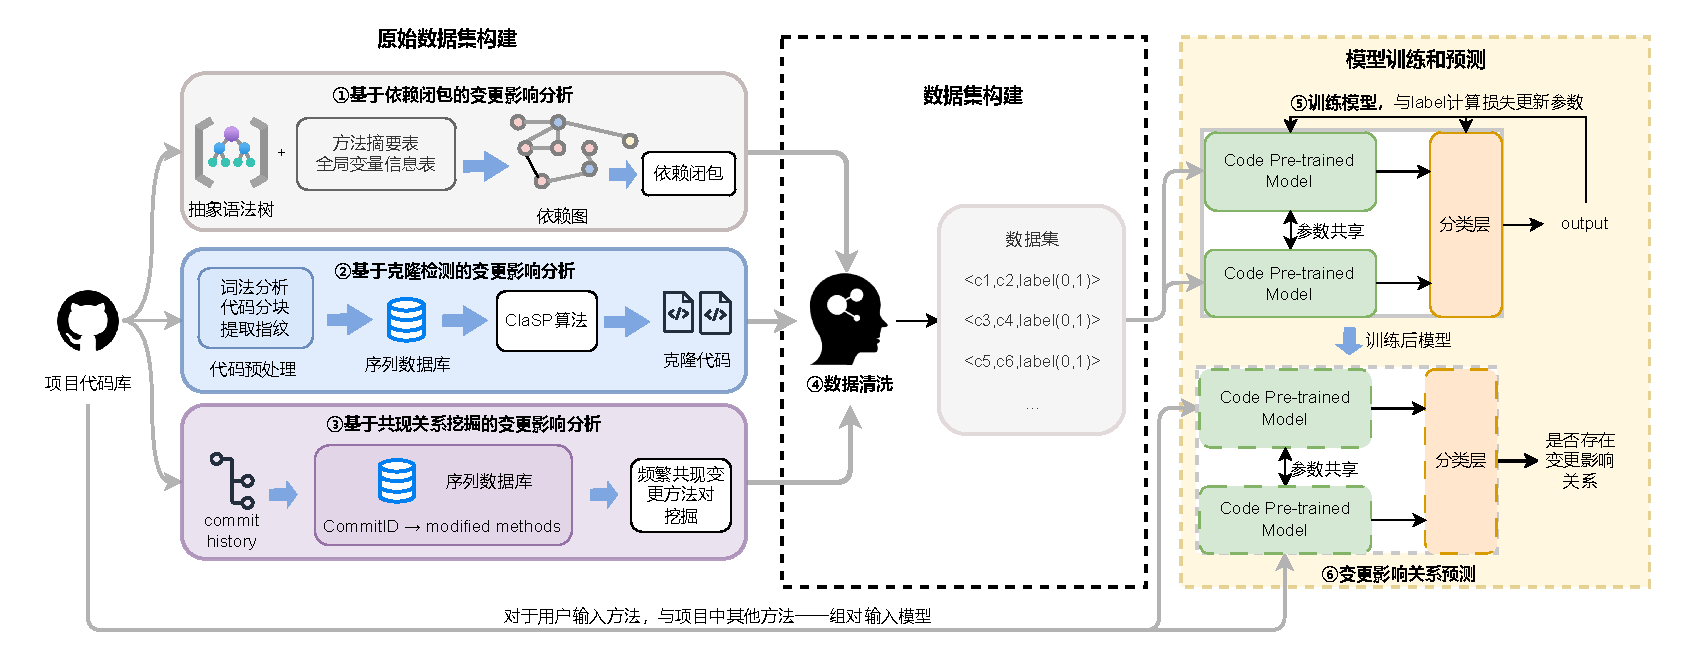
\includegraphics[width = 1\textwidth]{figures/2_预训练模型.pdf}
\caption{基于代码预训练模型的变更影响预测方法框架}
\label{2_基于代码预训练模型的变更影响预测方法框架}
\end{figure}

该方法的主要流程分为三步:(1)原始数据集构建。通过前文所述的依赖闭包、克隆检测和共现关系挖掘方法得到原始正例方法对。(2)构建精确数据集。对原始数据集进行数据清洗,排除数据集中误报的样例,并通过随机采样的方式构建负例方法对。(3)变更影响关系预测。首先对模型进行训练微调,然后使用微调后的模型进行预测,预测时对于用户输入的方法,遍历项目内所有方法,组对一一输入模型,得到与输入方法存在变更影响的方法列表。



\subsection{数据集来源和数据清洗}
\label{1_数据集来源和数据清洗}


\noindent \textbf{1. 数据集来源}

为了确保代码预训练模型能够有效识别依赖型和逻辑型两种变更影响关系,本文利用依赖闭包、克隆检测和共现关系挖掘方法生成的数据作为原始数据集。具体来说:(1)正例样本:从上述方法检测到具有变更影响关系的方法对中提取。(2)负例样本:在项目中随机采样一部分不具有变更影响关系的方法对,确保正负样本比例的平衡。

通过这种方式构建数据集,不仅能够覆盖多种影响关系,还为模型提供了明确的正负分类基础,有助于提高模型的识别能力。

\noindent \textbf{2. 数据清洗}

原始数据中可能包含噪声样本,例如依赖闭包方法生成的依赖方法对未必都具有变更影响关系,而共现关系挖掘方法中的支持度较低样本(如支持度为2)可能因偶然共现而导致误报。这些噪声数据会降低模型的训练效果,因此需要进行严格的数据清洗。

\begin{figure}[htbp]
\centering
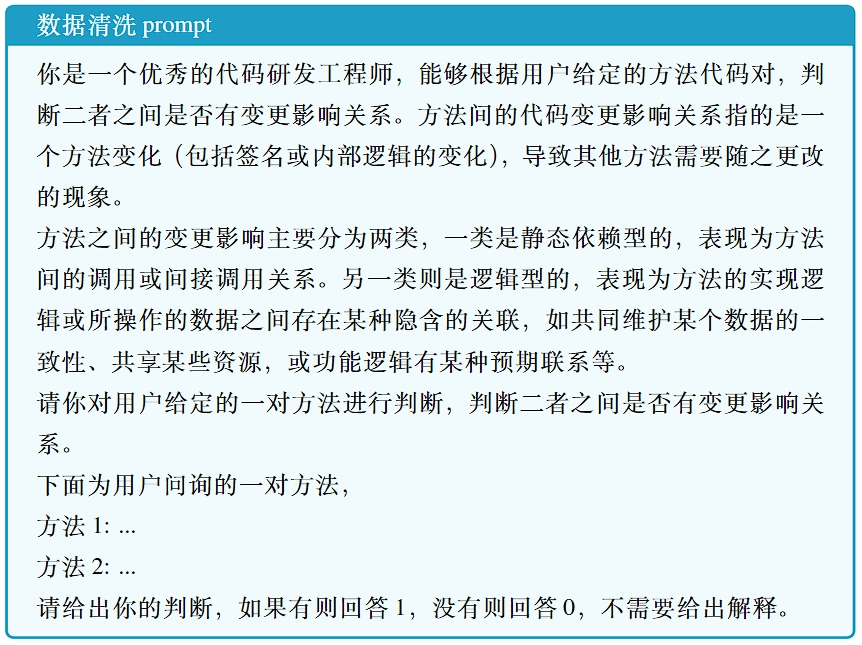
\includegraphics[width = 0.85\textwidth]{figures/1_数据清洗.png}
\caption{数据清洗所使用的的Prompt}
\label{1_数据清洗}
\end{figure}

为提高数据质量,本文结合当前主流的大语言模型(Large Language Model,LLMs)进行数据清洗。商业化大语言模型拥有较强的代码语义理解能力,可以通过推理较为准确地识别真实的变更影响关系。具体清洗步骤分为三步:(1)Prompt设计:为大语言模型提供明确的提示,包括变更影响关系的定义及其可能的表现形式,指导模型对样本中方法间的关系进行语义推理。(2)样本过滤:根据模型推理结果,过滤掉那些可能因误报产生的噪声样例。(3)验证数据一致性:通过对模型输出进行人工抽样验证,确保清洗后的数据集具有较高的准确性和可靠性。


图\ref{1_数据清洗}展示了本文用于数据清洗的Prompt设计。通过结合大语言模型的推理能力,本文显著提高了数据集的质量,为后续模型训练奠定了坚实基础。


\subsection{基于代码预训练模型的变更影响关系预测}

本文提出基于代码预训练模型的变更影响关系预测方法。首先需对代码预训练模型进行微调,训练后得到模型用于预测。该任务的输入为两个方法体,输出为两个方法之间是否存在变更影响关系,即“存在”或“不存在”。考虑到代码理解的复杂性与深度,相比于通用领域的如Bert,T5等预训练语言模型,面向代码领域进行预训练的CodeBert模型更适合作为编码器提取代码的表示。CodeBERT 是一种专为程序代码设计的预训练语言模型,通过大规模的代码语料库预训练,能够学习到代码中的丰富语法结构和语义信息。

\noindent \textbf{1. 训练过程}

首先需要对模型进行训练,微调代码预训练模型的参数,训练分类模型的参数,整个模型架构如图\ref{1_code_bert_overall}所示,主要分为两部分,分别是代码表示模块和融合分类模块。代码表示模块为CodeBert,融合分类模块包括拼接融合和分类两个过程。接下来对模型的各个步骤进行详细介绍。
\vspace{0mm}
\begin{figure}[h]
\centering
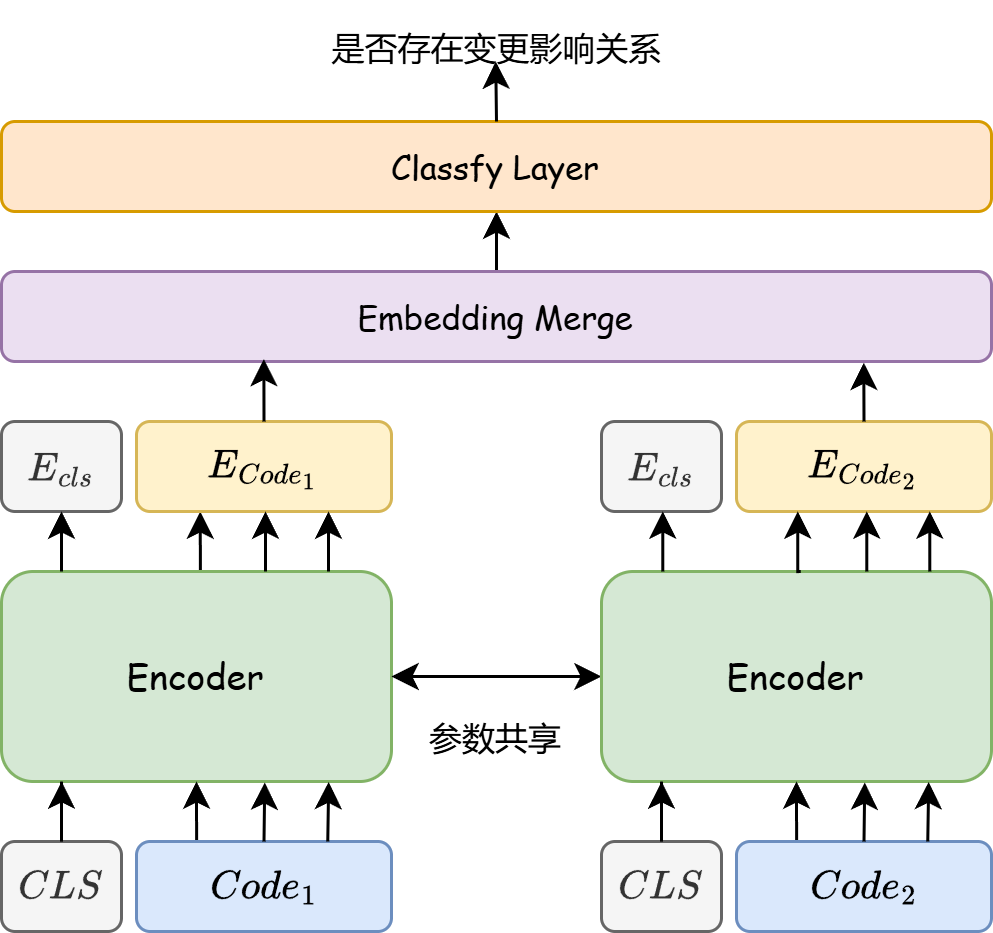
\includegraphics[width = 0.70\textwidth]{figures/1_code_bert_overall.png}
\caption{基于代码预训练模型的算法架构}
\label{1_code_bert_overall}
\end{figure}


首先,将两个方法体$ Code_1, Code_2$,先通过代码预训练模型进行编码
\begin{align}
H_{Code_1}=&Encoder(Code_1) \in \mathbb{R}^{(len,dim)} \\
E_{Code_1}=&mean(H_{Code_1}[1:...]) \in \mathbb{R}^{(dim)}
\end{align}

其中$len$表示$Code_1$的序列长度,$dim$为Encoder的隐层表示维度,得到方法的向量化表示$ E_{Code_1}, E_{Code_2}$。

通过拼接融合这两个向量,得到融合后向量表示$E_{Code_1,Code_2}$
\begin{align}
E_{Code_1,Code_2}=Concat& (E_{Code_1},E_{Code_1})\in \mathbb{R}^{(dim*2)} 
\end{align}

将融合后的向量表示送入一个由两层组成的多层感知机(Multilayer Perceptron,MLP)中,再通过 softmax 层进行分类处理,将模型的输出转化为一个概率分布,表示两个方法体之间存在关系的概率。
\begin{align}
logits_{Code_1,Code_2}=MLP(E_{Code_1,Code_2})&=FFN(ReLU(FFN(E_{Code_1,Code_2}))) \\
FFN(x)&=Wx+b\\
ReLu(x)&=max(0,x)\\
logits_{Code_1,Code_2}& \in \mathbb{R}^{(2)}
\end{align}

其中,$logits_{Code_1,Code_2}$为模型的MLP层最后给出的两种标签(存在关系,不存在关系)各自的概率。
\begin{align}
loss=CrossEntryLoss(logits_{Code_1,Code_2}, Label)
\end{align}

与真实标签$Label$计算交叉熵损失,得到loss,计算梯度,优化模型参数。

\noindent \textbf{2. 预测过程}

经过训练得到的模型即可用于预测。预测的过程同训练的过程类似,主要包括以下步骤:(1)对于用户输入的单个方法,遍历项目中的其他方法,分别与用户输入方法组对输入模型。(2)经过编码模块CodeBert得到代码的向量表示。经过 CodeBERT 模型的表示学习过程,所得到的向量不仅包含了每个方法体的语法特征,还能编码代码中的语义关系及其他潜在的编程特征。(3)融合并分类。通过拼接融合两个向量,通过分类层进行分类,得到存在和不存在变更影响关系的概率分布,概率较大的即为预测结果。


\section{实验结果与分析}

\subsection{实验数据}

\noindent \textbf{1. 实验数据来源}

本文从影响力或社区活跃程度的角度出发,收集了表\ref{1_data_from}中所示的软件项目为被测项目进行实验。这些项目在github上的收藏数均在千以上,说明这些项目在开源社区中有着一定的影响力,使用范围比较广泛。除antiword之外,这些项目还有着比较活跃的社区,说明其还在不断更新迭代过程中,因此能提供较为丰富的变更历史,以供共现关系挖掘方法的实验分析。

\begin{table}[htbp]
\caption{被测项目}
\label{1_data_from}
\vspace{0.5em}\centering\wuhao
\begin{tabular}{cp{6cm}ccc}
\toprule
项目名称 & 项目简介 & 代码行数& 提交数 & 收藏数 \\
\midrule
TheAlgorithms & 各种算法的开源实现,涵盖了计算机科学、数学和统计学等领域 & 24645 & 1536 & 57k \\
antiword-0.37 & 提取 Microsoft Word 文档内容的工具 & 34725& - & 13k\\
jemalloc-5.3.0 & 通用的malloc(3)实现,强调碎片避免和可扩展的并发支
持  &83525& 3530 & 9k \\
libbpf-1.1 & linux 内核观测技术的一个脚手架库 & 127927 & 2375 & 1.9k \\
librdkafka-2.1.0& Apache Kafka 的 C/C++ 客户端库 & 154951 & 4430 & 18k \\
FFmpegKit-5.1.0 & FFmpeg 工具包 & 450998 & 369 & 3.7k \\

\bottomrule
\end{tabular}
\end{table}

\noindent \textbf{2. 训练数据}

基于代码预训练模型的变更影响预测方法的训练数据集收集方式如\ref{1_数据集来源和数据清洗}节所述,数据清洗过程中使用的模型为 Doubao (API model name:Doubao-lite-32k-240428),为了保证测试集和训练集的不重叠性,在经过收集和清洗后得到的关系中排除测试变更点。得到的训练数据统计信息如表\ref{1_数据集统计信息1}所示,共12156对数据。

\begin{table}[htbp]
\caption{训练数据统计信息}
\label{1_数据集统计信息1}
\vspace{0.5em}\centering\wuhao
\begin{tabular}{cccc}
\toprule
项目名称 & 正例对数 & 负例对数 & 总对数 \\
\midrule
TheAlgorithms    & 297 & 500 & 797 \\
antiword-0.37    & 230 & 500  & 730 \\
jemalloc-5.3.0   & 993 & 2000 & 2993 \\
libbpf-1.1       & 801 & 1500 & 2301 \\
librdkafka-2.1.0 & 1432  & 3000 & 4432 \\
FFmpegKit-5.1.0  & 303 & 600 & 903 \\ 
总计              & 4056 & 8100 & 12156 \\
\bottomrule
\end{tabular}
\end{table}


\noindent \textbf{3. 测试数据}

根据每个示例项目的上一个版本和示例版本间的版本变更,各自随机选取30个方法作为变更方法,以代码变更历史作为辅助,以半手工的方式进行标注,得到真实的被影响方法集AIS(Actual Impact Set)作为测试集,这里分别统计了依赖型和逻辑型的变更影响关系,得到的数据如表\ref{1_test_data_info}所示。再分别通过前述方法进行检测,得到估计的被影响方法集EIS(Estimated Impact Set),通过评价指标评估方法的有效性。

\begin{table}[htbp]
\caption{测试数据统计信息}
\label{1_test_data_info}
\vspace{0.5em}\centering\wuhao
\begin{tabular}{cccccc}
\toprule
项目名称  & 变更点数 & 依赖型AIS & 逻辑型AIS & 总计 \\
\midrule
TheAlgorithms  & 30 & 98 & 21 & 119\\
antiword-0.37  & 30 & 119 & 54 & 173 \\
jemalloc-5.3.0   & 30 & 67 & 14 & 81 \\
libbpf-1.1  & 30 & 194 & 17 & 211 \\
librdkafka-2.1.0  & 30 & 92 & 26 & 118\\
FFmpegKit-5.1.0  & 30 & 105 & 17 & 122\\
总计  & 180 & 675 & 149 & 824 \\
\bottomrule
\end{tabular}
\end{table}


\subsection{评价指标}\label{1_评价指标}

真实的被影响方法表示为AIS,每种方法检测得到的结果为估计的被影响方法EIS,按逻辑型和依赖型对关系进行划分,根据这两个值计算精确度、召回率和F-measure,这三种评价指标在信息检索的场景下被广泛使用,本章中用于评价变更影响分析方法的有效性。
\begin{align}
precision &= \frac{|EIS \cap AIS|}{|EIS|} 
\end{align}

\begin{align}
recall &= \frac{|EIS \cap AIS|}{|AIS|}  
\end{align}

\begin{align}
F-measure &= \frac{2 \times precision \times recall}{precision + recall} 
\end{align}


\subsection{实验设置}

代码预训练模型选择:本文使用了CodeBERTa-small-v1\cite{husain_codesearchnet_2019}和codebert-base-mlm\cite{feng2020codebert}两个模型分别作为代码表示模型,得到的代码表示为768维,融合两组表示后使用的多层MLP的维度为768*2,64,2。 骨干模型的学习率设置为1e-5,分类器的学习率设置为5e-4,优化器Adam的两个参数 $\beta_1$,$\beta_2$分别设置为0.95,0.999,batch\_size 为 64。数据收集过程中,共现关系挖掘方法置信度设为1,支持度设为2以获得较多的训练原始数据。

在实际训练过程中,由于CodeBERTa-small-v1和codebert-base-mlm模型都是类Bert模型,允许输入的上下文长度最大为512,但是经过统计数据集中有67\%左右的方法体在分词之后的Token数量是大于512的,所以本实验在实验中对于超长的方法体按照512进行分片,分片进行编码后对多组分片的$CLS$ token的表示进行平均,来作为方法体的编码表示。

实验使用 PyTorch \cite{paszke2019pytorch} 和 Transformer 库 \cite{wolf2020transformers}  实现。模型CodeBERTa-small-v1和codebert-base-mlm均在单个 NVIDIA Tesla V100 GPU 上训练。


\subsection{实验结果与对比分析}

本节将通过实验对比来评估本章中提出的基于代码预训练模型的变更影响预测方法的性能,这里主要讨论下列三个问题:

RQ1:本章提出的基于代码预训练模型的方法能否有效检测变更影响关系?与其他方法相比,它在精确率,召回率和F-measure上表现如何?

RQ2:四种方法在提取依赖型(Dependence-Based)和逻辑型(Logic-Based)的变更影响关系上各自的优势如何?尤其是对于逻辑型的影响关系的检测是否足够全面?分别适用于哪些特殊场景?又各自有怎样的局限性?

RQ3:基于代码预训练模型的方法的跨项目迁移表现如何?针对不同代码风格、结构和质量的项目,模型是否能是否能够保持较高的准确性和稳定性?

\textbf{1.针对于RQ1的实验}

四种方法的实验结果如表\ref{1_变更影响实验结果}所示。总的来讲,两个基于代码预训练模型的方法表现最好,其F-measure在所有方法中表现最优,并且在查全和查准的能力上较为平衡。这说明基于代码预训练模型的方法能够学习到过去变更历史中的行为模式,并能将学习到的变更关系知识进行迁移,用于判断新的影响关系。

\begin{table}[htbp]
\caption{变更影响实验结果}
\label{1_变更影响实验结果}
\vspace{0.5em}\centering\wuhao
\begin{tabular}{cccccccc}
\toprule
方法 & F-measure(\%) & recall(\%) & precision(\%)  \\
\midrule
依赖闭包 & 36.8&81.9&23.7  \\
克隆检测 & 3.8&2.3&11.6 \\
共现关系挖掘 & 52.8&42.3&\textbf{70.4} \\
依赖$\cup$克隆$\cup$共现 & 47.1&\textbf{88.4}&32.1 \\
codebert-base-mlm & 58.8&53.9&64.8 \\
CodeBERTa-small-v1 & \textbf{59.5} & 55.3 & 64.4 \\
\bottomrule
\end{tabular}
\end{table}

基于依赖闭包的方法表现为召回率较高而准确率很低,仅为23.7\%。这是由于依赖闭包方法本身的特性决定的,由于变更影响关系随涟漪扩散效应,越向外扩散影响越小,但该方法却平等地认为扩散所至的代码均存在影响关系,这会导致较多误报。

\begin{figure}[htbp]
\centering
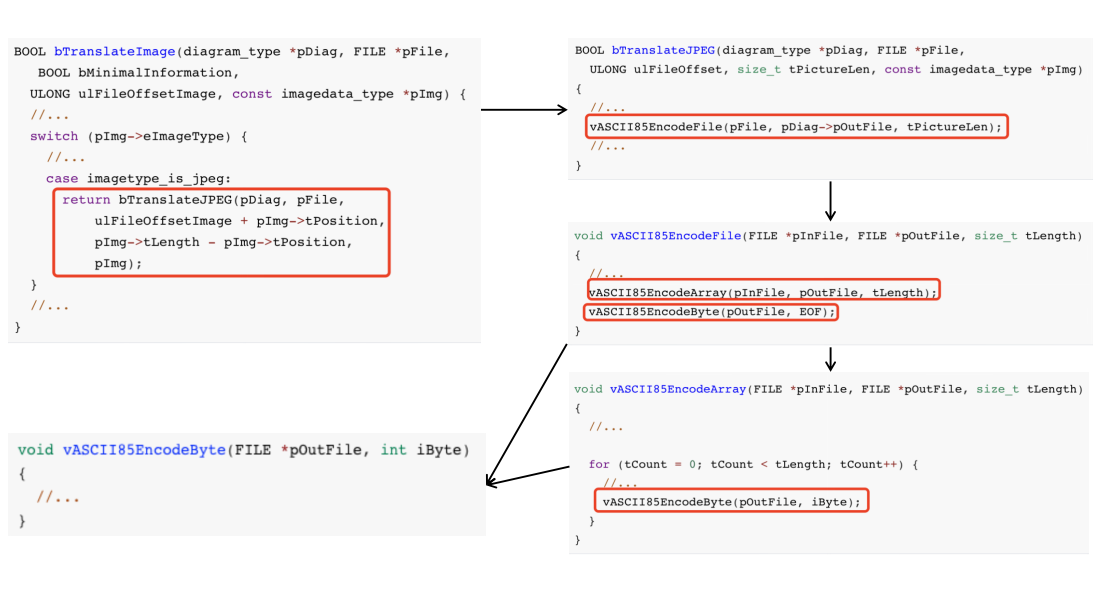
\includegraphics[width = 0.95\textwidth]{静态分析拒绝样例.jpg}
\caption{依赖闭包方法迭代路径}
\label{1_依赖闭包方法迭代路径}
\end{figure}

如在图\ref{1_依赖闭包方法迭代路径}中所示是antiword项目中从bTranslateImage方法出发得到的部分依赖图,它层层递进地展示了从word中提取jpec图片的过程,bTranslateImage调用bTranslateJPEG,处理jpec图片,再调用vASCII85EncodeFile,将图片提取为文件,再依次调用vASCII85EncodeArray和vASCII85EncodeByte。当对Byte方法进行变更影响分析时,根据RETURN关系的涟漪效应,最终会将图中所示的其他4个方法都列为影响集。然而实际上,该方法只对\{Array, File\}存在变更影响关系,最显然的,当Byte方法的签名发生改变时,将直接影响到\{Array, File\},这两个方法如果不更改将发生编译错误。而对另两种方法的影响则微乎其微。

其次基于共现关系挖掘的方法的准确率较高,但召回率略低。这表明,代码变更历史中方法的共现关系的确蕴含了大量能够有效揭示变更影响关系的信息。这是因为变更历史中都是前人对软件项目进行变更的记录,这样的提交由开发者精确变更,并经历过开源项目中非常严格的审查过程才合入主分支,因此较为准确地反映了代码变更中的实际操作,从而也能将过去的开发模式反映在共现关系挖掘的结果集中。但是由于一些代码并未存在变更,因此该方法忽略了部分较为稳定的代码之间的变更影响关系,导致了一定程度的漏报。

基于代码克隆检测的方法则整体效果最差。这是由于该方法只能准确的识别由于克隆关系产生的变更影响,而在质量良好的项目代码中,克隆代码的现象很少出现,因此提取到样例本身也较少,就导致其整体效果不佳。在实践中,建议基于克隆关系的方法作为其他方法的补充使用。本文进一步将三种方法进行结合,尽管结合后召回率为最高,但整体效果表现依旧是基于代码预训练模型为最佳。

\textbf{2.针对于RQ2的实验}

RQ1中从整体的角度上说明了三种方法的有效性。为了回答RQ2,这里对每种方法检测得到的依赖型(Dependence-Based)和逻辑型(Logic-Based)的变更影响关系分别进行计算,得到如表\ref{1_两类变更影响关系实验结果}的结果,通过对比能更直观地发现不同方法的优势和特点。


\begin{table}[htbp]
\caption{两类变更影响关系实验结果}
\label{1_两类变更影响关系实验结果}
\vspace{0.5em}\centering\wuhao
\begin{tabular}{c|ccc|ccc}
\toprule
  & \multicolumn{3}{c|}{Dependence-Based} & \multicolumn{3}{c}{Logic-Based}  \\
\midrule
方法 & F-measure & recall & precision & F-measure & recall & precision  \\
\midrule
依赖闭包 &  44.8 & 100 & 28.9 & - & - & -  \\
克隆检测 &  - & - & - & 31.8 & 19.1 & 95.7 \\
共现关系挖掘 &  56.0 & 44.6 & 75.4 & 57.0 & 47.3 & 71.8 \\
依赖$\cup$克隆$\cup$共现 &  44.1 & 100 & 28.3 & 62.3 & 53.7 & 74.1 \\
codebert-base-mlm &   61.2 & 55.1 & 68.9 & 70.9 & 72.6 & 69.3 \\
CodeBERTa-small-v1 &   \textbf{61.9} & 56.6 & 68.3 & \textbf{71.7} & 73.9 & 69.7 \\
\bottomrule
\end{tabular}
\end{table}

\textbf{(1)依赖闭包方法} \hspace{2mm}对于依赖型影响没有漏报,但依赖型影响关系的误报较高,导致依赖型的检测表现整体上较差。针对逻辑型的变更,该方法则无法检测到,这是由于逻辑型的影响关系无法在依赖图中产生联系,因此依赖闭包方法无法检测。

\textbf{(2)克隆检测方法} \hspace{2mm}逻辑型影响几乎没有误报,其准确率能达到95.7\%,说明其非常擅长挖掘逻辑型中由于克隆代码导致的变更影响关系。但其缺点在于仅能检测检测由于代码克隆导致的逻辑型影响,对于其他逻辑型和依赖型影响存在严重漏报。

\begin{figure}[h]
\centering
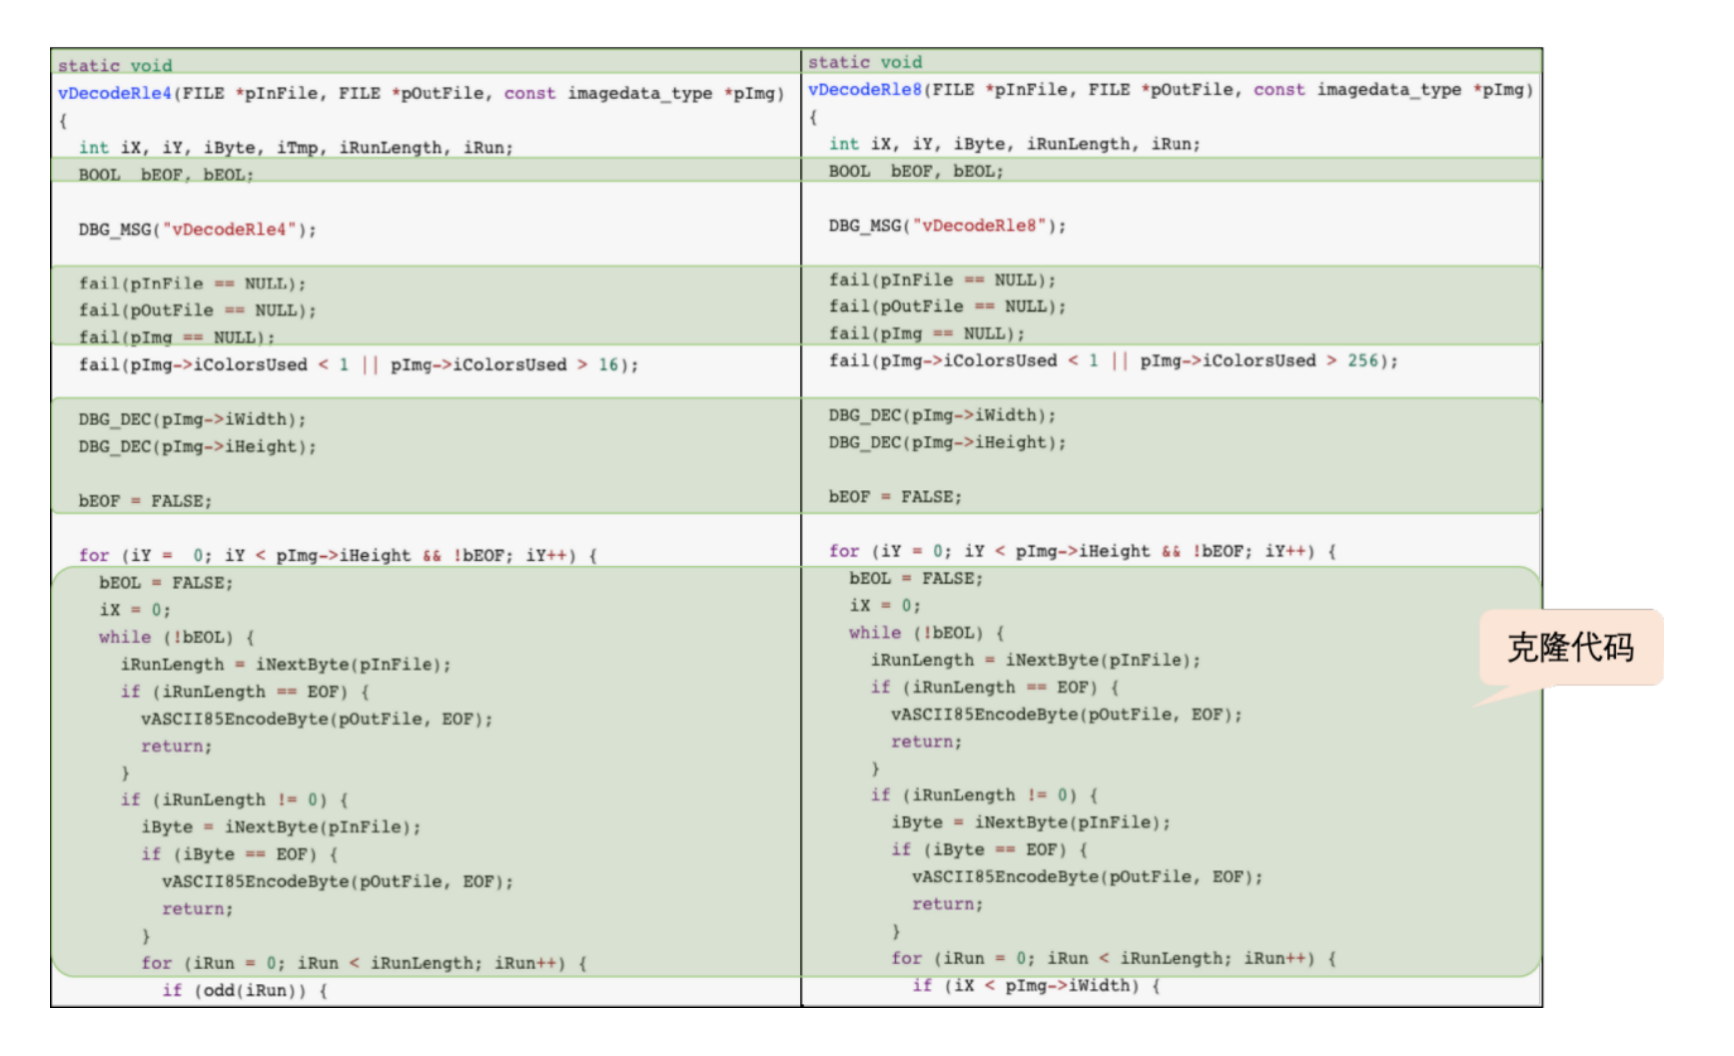
\includegraphics[width = 1\textwidth]{克隆代码示例.jpg}
\caption{包含克隆代码片段的一组方法实例}
\label{1_包含克隆代码片段的一组方法实例}
\end{figure}
    
为说明克隆检测方法的优势,以其检测到的一对有变更影响关系的方法为例,如图\ref{1_包含克隆代码片段的一组方法实例}所示。这里展示了这对方法的部分代码,其中绿色高亮的部分表示代码克隆的区域。这两个方法的主要功能是分别对8位和4位压缩格式的图像进行解码。我们发现,这对方法中的大部分逻辑结构几乎完全相同,只有少部分关键处理逻辑存在差异。由此,我们可以认定,这两个方法的变化过程很可能是同步的,即在实际的维护过程中,当对其中一个方法进行修改时,另一个方法也通常需要同步进行相应的变更,才能保证逻辑的一致性。



这种现象表明,在软件的演化过程中,维护人员可能需要对这两个方法进行联动更新。任何对其中一个方法的修改都可能影响到另一个方法的功能或逻辑一致性,在代码维护时必须考虑它们之间的相互依赖关系。而克隆检测方法能准确检测出此种影响。

\textbf{(3)共现关系挖掘方法} \hspace{2mm}该方法对两种类型的变更影响关系均可检测,且综合表现优于依赖闭包和克隆检测方法。以该方法在 librdkafka 项目中检测到的一对方法为例,如图 \ref{1_逻辑上有变更影响关系的方法对示例-incr和decr} 所示,该项目是 Apache Kafka 的一个高性能 C/C++ 客户端库,左侧的方法rd\_kafka\_global\_cnt\_decr负责对计数器进行减一操作,而右侧的方法rd\_kafka\_global\_cnt\_incr则负责对计数器进行加一操作。

\begin{figure}[h]
\centering
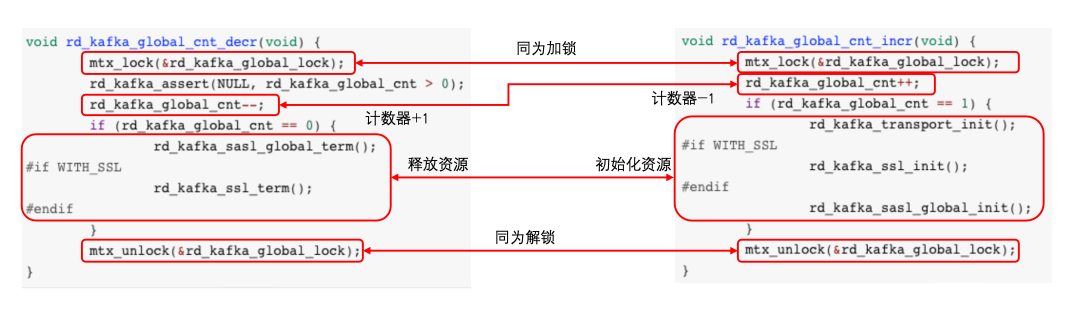
\includegraphics[width = 1\textwidth]{incrdec.jpg}
\caption{逻辑上有变更影响关系的方法对示例-incr和decr}
\label{1_逻辑上有变更影响关系的方法对示例-incr和decr}
\end{figure}

这两个方法是一对典型的协作方法。incr 方法负责计数器加一并在计数器从零变为一时初始化资源,而 decr 方法则在计数器减为零时释放资源。尽管它们在依赖图上没有直接联系,但由于在功能上互为补充,共同承担了计数器的管理和资源的初始化与释放工作,表现出“镜像”特性。因此若一个方法的实现逻辑发生变化,另一个方法通常也需相应调整,以保持逻辑一致性。这种变更影响关系属于典型的逻辑关联型,体现了该方法在检测逻辑型影响的优秀潜力。

但该方法也存在一定局限性:(1)要求项目代码必须有变更历史。(2)挖掘算法的支持度会影响结果。表\ref{1_支持度对共现关系挖掘方法的影响}展示了支持度分别为2和3时的实验结果。可以看出,支持度越大,误报减少,但漏报增多。这表明,较高的支持度能排除偶然共现的影响,但会限制影响关系的普遍性,导致检测到的关系减少,从而增加漏报。(3)挖掘到的信息属于硬信息。仅依靠变更历史的只能得到变更过的方法之间影响,未变更过或变更次数较少的影响关系无法反映,相同的影响模式之间无法进行迁移。
        
\begin{table}[htbp]
\caption{支持度对共现关系挖掘方法的影响}
\label{1_支持度对共现关系挖掘方法的影响}
\vspace{0.5em}\centering\wuhao
\begin{tabular}{c|ccc|ccc}
\toprule
  & \multicolumn{3}{c|}{Dependence-Based} & \multicolumn{3}{c}{Logic-Based}  \\
\midrule
方法 & F-measure & recall & precision & F-measure & recall & precision  \\
\midrule
共现关系挖掘-支持度-2 & 55.5 & \textbf{51.2} & 60.7 & 56.1 & \textbf{58.9} & 53.5 \\
共现关系挖掘-支持度-3 & \textbf{56.0} & 44.6 & \textbf{75.4} & \textbf{57.0} & 47.3 & \textbf{71.8} \\
\bottomrule
\end{tabular}
\end{table}

\textbf{(4)基于代码预训练模型方法} \hspace{2mm}该方法在两类变更影响关系上的表现均达到最优,与之前的方法相比,在两类变更影响关系上的F-measure分别提升了5.9\%和14.7\%。该方法有效解决了共现关系挖掘方法在缺乏变更历史时的冷启动问题,且在逻辑型影响的挖掘上能够实现影响模式的迁移。

然而,该方法在依赖型影响的检测上虽也有提升,但相对于逻辑型影响来说,提升效果较为有限,经过分析发现可能是由于该方法仅依靠两个方法体的特征向量进行预测,不管是直接依赖还是逻辑型依赖,在代码中都存在较为明显的特征,而间接依赖的方法对之间,特征则微乎其微,中间的依赖信息丢失了。因此这样的方法体之间在语义层面的关联性较难识别,从而导致对这种类型依赖关系的识别能力较弱。

此外,由于该方法仅通过方法体对变更影响关系进行预测,因此在实际使用中需要对项目中的所有两两方法的组合进行计算。以antiword项目为例,该项目中共有578个方法体,测试集中的变更点为30个。对于每一个变更点,都需要与项目中的所有方法进行一一比对,计算的次数为30 * (577) = 17,310次,每次计算均需要通过嵌入和分类过程。大量的计算时间消耗显著影响了该方法的可用性,从而限制了其在大规模项目中的应用效果。
    

\textbf{3.针对于RQ3的实验}

为了探索基于代码预训练模型在跨项目方面的迁移能力,本节对实验所使用到的训练数据按项目进行划分。跨项目实验仅使用训练集中属于TheAlgorithms,antiword-0.37,librdkafka-2.1.0和FFmpegKit-5.1.0这四个项目的数据进行训练,测试集与前述实验相同。在训练集中的四个项目训练后测试的结果称为项目内测试结果(Intra-Project Testing),jemalloc-5.3.0和libbpf-1.1则是项目间测试结果(Inter-Project Testing)。这样的训练方式使其更符合应用时的场景设置,即在使用时可能会遇到训练中从未见过的项目。


\begin{table}[htbp]
\caption{跨项目迁移能力分析(F-measure(\%))}
\label{1_跨项目迁移能力分析}
\vspace{0.5em}\centering\wuhao
\begin{tabular}{c|cccccc}
\toprule
方法& TheAlgorithms & antiword & librdkafka & FFmpegKit & jemalloc & libbpf\\
\midrule
train on 6 datasets & \multicolumn{6}{c}{Intra-Project Testing} \\
\midrule
codebert-base-mlm &  59.66 & 60.43 & 57.47 & 57.03 & 59.67 & 57.82\\
CodeBERTa-small-v1 &  60.23 & 59.64 & 60.18 & 57.87 & 60.99 & 58.22\\
\midrule
train on 4 datasets & \multicolumn{4}{c|}{Intra-Project Testing} & \multicolumn{2}{c}{Inter-Project Testing} \\
\midrule
codebert-base-mlm &   61.72 & 61.55 & 62.03 & \multicolumn{1}{c|}{60.65} & 42.49$^*$ & 39.75$^*$ \\
CodeBERTa-small-v1 &  62.28 & 65.24 & 63.45 & \multicolumn{1}{c|}{62.19} & 41.92$^*$ & 40.8$^*$\\
\bottomrule
\end{tabular}
\end{table}

实验结果如表\ref{1_跨项目迁移能力分析}所示,在特定项目上进行训练的模型,其在对应的测试集上的表现略有提升,在项目间的测试集上也能有一定的性能迁移,但相比在六个项目上进行训练的模型,性能下降在28.9\% 到 31.7\%之间。

\textbf{4.方法对比总结}

上述四种方法为检测代码变更影响关系提供了多样化的解决方案。每种方法在处理不同类型的变更影响关系时各有侧重,适应于不同的应用场景。然而每种方法也存在一定的局限性。对于这些方法的比较与总结,请参见表\ref{1_变更影响分析方法对比总结}。

\clearpage


\begin{table}[htbp]
\caption{变更影响分析方法对比总结}
\label{1_变更影响分析方法对比总结}
\vspace{0.5em}\centering\wuhao
\begin{tabular}{c|c|p{4cm}|p{4cm}}
\toprule
方法& 检测关系 & 优势 & 局限性\\
\midrule
依赖闭包 & 依赖型 & 依赖型漏报低 & 依赖型误报高,且仅能检测依赖型\\
\midrule
克隆检测 & 逻辑型-代码克隆 & 逻辑型中克隆关系影响的误报低 & 只能检测代码克隆一种关系\\
\midrule
共现关系挖掘  & 依赖型和逻辑型 & 两类影响的性能均较好 & 无法应用于没有变更历史的项目,不频繁变更无法被检测 \\
\midrule
代码预训练模型  & 依赖型和逻辑型 & 两类影响的性能均较好 & 计算效率问题,间接依赖丢失问题 \\
\bottomrule
\end{tabular}
\end{table}



\section{本章小结}

本章实现了基于依赖闭包、克隆检测、共现关系挖掘的变更影响分析方法,并提出了基于代码预训练模型的变更影响预测方法。通过实验分析了基于依赖闭包、克隆检测、共现关系挖掘的三种方法的优势以及局限性,实验中基于代码预训练模型的变更影响预测方法在两大类关系的检测中均表现出了最优的性能,并且各个指标上没有明显缺陷,但是由于其对计算量的要求较高,所以在实际场景中的应用价值会有一定程度的折扣。

% Local Variables:
% TeX-master: "../main"
% TeX-engine: xetex
% End:
